\documentclass{../paper}

\newcommand{\todo}[1]{\textcolor{red}{To-do: #1}}

\begin{document}

\title{Muon Physics \\ {\em Post-lab}}

\author{Iago B.~Mendes\,\orcidlink{0009-0007-9845-8448}}
\email{ibrazmen@oberlin.edu}
\affiliation{Department of Physics and Astronomy, Oberlin College, Oberlin, Ohio 44074, USA}

\date{\today}

\maketitle

\section{Background}

Primary cosmic rays (made out of mostly protons) interact with the nuclei of air molecules in the upper atmosphere, creating additional particles. Among these extra particles, we find pions that spontaneously decay into muons as
\begin{equation}
  \pi^+ \to \mu^+ + \nu_\mu
\end{equation}
or
\begin{equation}
  \pi^- \to \mu^- + \bar\nu_\mu.
\end{equation}
The resulting muons then travel down to sea level, where we can detect them. When slowed down, these muons decay into electrons,
\begin{equation}\label{eq:muon-decay}
  \mu^- \to e^- + \bar\nu_e + \nu_\mu,
\end{equation}
or positrons,
\begin{equation}\label{eq:muon+decay}
  \mu^+ \to e^+ + \nu_e + \bar\nu_\mu.
\end{equation}

Note that we do not have to account for the time it takes the muon to travel from the upper atmosphere to sea level when calculating the muon's lifetime. We only need to measure the time that muons stay in our detector. If we measure many of these in-detector times, the distribution should follow the same exponential decay $e^{-t/\tau}$ as in the number of muons per time after creation $N(t)$, allowing us to find the muon's lifetime $\tau$.

\section{Procedure}

To measure the lifetime of the muon, we use a plastic scintillator. The detector works by measuring the decay of muons that stop inside it. When a muon enters the scintillator, it slows down and eventually stops, emitting a pulse of scintillation light, which triggers a timing clock \cite{TeachSpinManual}. The muon then decays according to \eqref{eq:muon-decay} or \eqref{eq:muon+decay}, resulting in a second pulse \cite{TeachSpinManual}. By comparing the time interval between these two pulses, we can determine how long the muon lived inside the detector.

The accuracy and precision of the detector are limited by two main factors. First, the time resolution of the detector limits the precise measurement of short time intervals. This time resolution issue is particularly relevant when fitting our data to a Gaussian, as highlighted in the next section. Second, background noise from cosmic rays and environmental radiation can introduce false signals in our data \cite{TeachSpinManual}. The detector addresses these false signals by limiting the time interval between the scintillation pulses. Specifically, the timing clock keeps waiting for a second pulse up to 20000 ns after the first one. If no second pulse is detected, the detector classifies this as a single event and discards the measurement.

Over the course of 20 seconds, we can estimate that 97 single events occur based on \cite{Sage}. That is, we have a rate of $\sim 5$ single events per second. Over the course of 599,405 seconds, we recorded 12,608 muon decays. That is, we have a rate of $\sim 0.02$ muon decay per second. Therefore, at each second, the probability of a muon stopping is $\sim 0.4\%$. This indicates that it is very unlikely that we will have more than one muon decay at a given time in the detector.

\section{Results}

\begin{figure*}
  \centering
  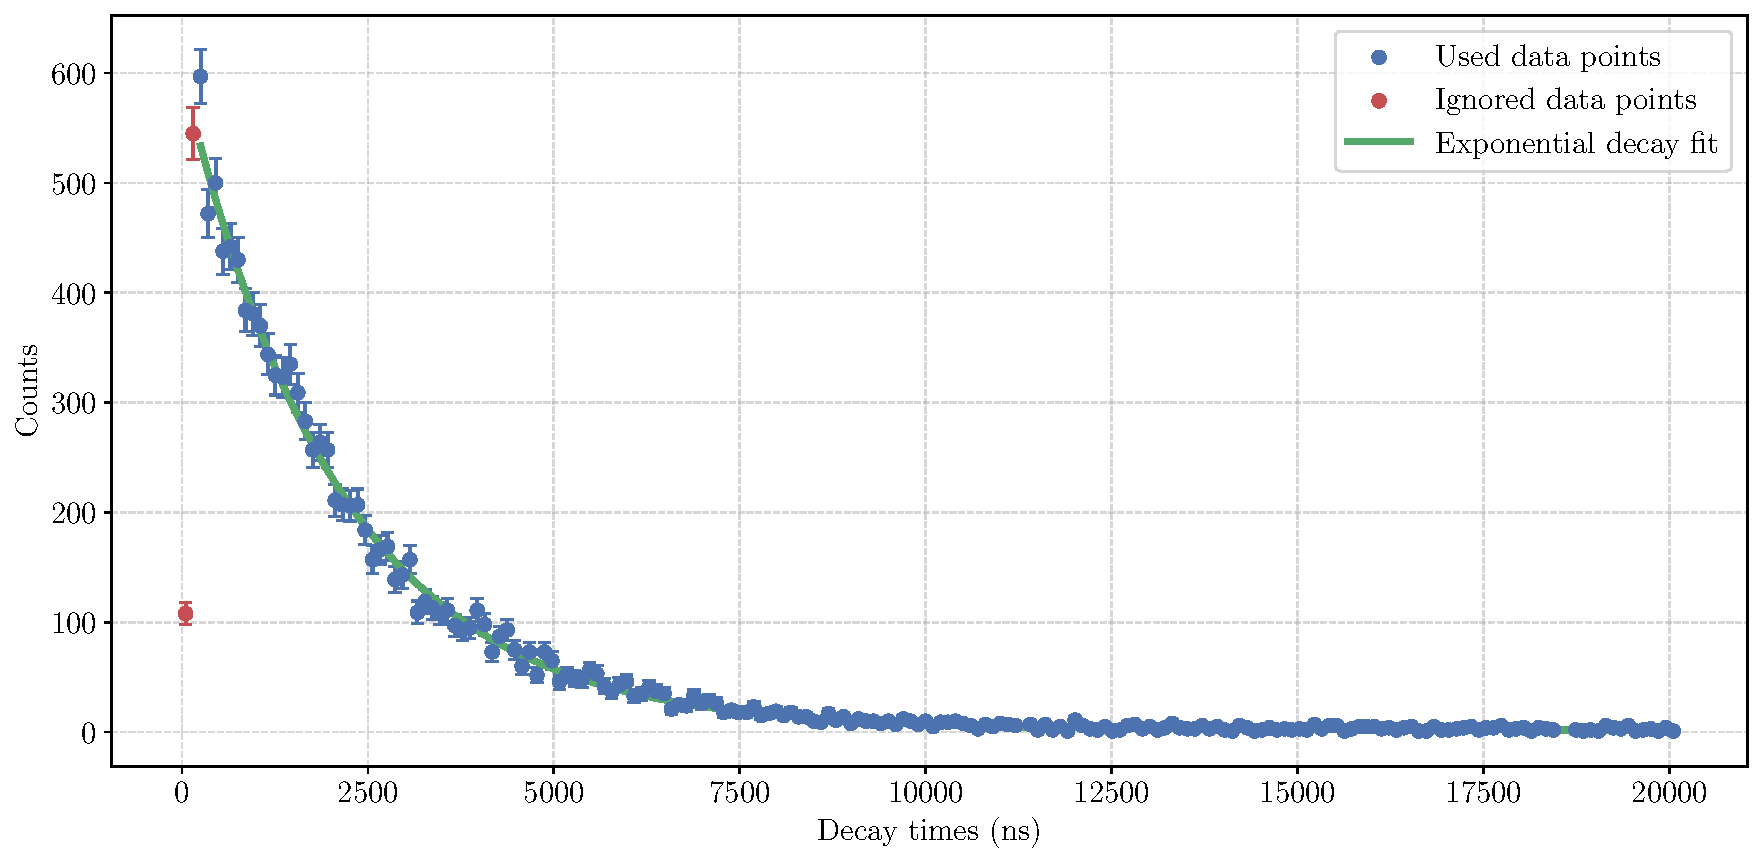
\includegraphics[width=\textwidth]{data/analysis.pdf}
  \caption{Histogram of muon decay times.}
  \label{fig:analysis}
\end{figure*}

A histogram of our measured decay intervals is shown in Figure \ref{fig:analysis}. To analyze find the best possible binning strategy of our data, we perform the following steps for each given number of bins $N$.
\begin{enumerate}
  \item Calculate bin width.
  \item Categorize data into bins.
  \item Remove any empty bins.
  \item Find bin with maximum count and ignore any bins before it.
  \item Calculate the uncertainty of each bin $i$ with $N_i$ counts as $\delta N_i = \sqrt{N_i}$.
  \item Use {\tt SciPy}'s {\tt curve\_fit} procedure \cite{SciPy} to fit our data as an exponential decay of the form
    \begin{equation}
      N(t) = A e^{-t/\tau} + C,
    \end{equation}
    where $A$ is the amplitude, $\tau$ is the timescale, and $C$ is a vertical offset.
  \item Calculate reduced chi squared $\bar\chi^2$.
\end{enumerate}

Note that step 4 is needed in order to address the time resolution limitation of the detector. By starting the fit at the bin with maximum count, we ignore bins at under-resolved times.

We performed steps 1--7 for all $50 \leq N \leq 500$ (at incremental steps of 5). We found the best reduced chi squared value,
\begin{equation}
  \bar\chi^2 = 1.007,
\end{equation}
with $N=200$ bins (out of which 195 bins remain after steps 3 and 4). With this, our measurement for the lifetime of the muon is
\begin{equation}\label{eq:muon-decay-value}
  \tau = 2.10(2) \ \mu\text{s}.
\end{equation}

It is important to note that negative muons interact with the atoms in the scintillator. Such interaction results in a spontaneous decay of the form
\begin{equation}
  \mu^- + p \to n + \nu_\mu
\end{equation}
\cite{TeachSpinManual}. Due to this other form of decay, we see a lower effective lifetime for $\mu^-$ compared to $\mu^+$ \cite{NIST_muon}. Hence, \eqref{eq:muon-decay-value} is a charge-averaged measurement of the lifetime of the muon. From \cite{TeachSpinManual}, we know that the literature lifetimes of $\mu^+$ and $\mu^-$ are
\begin{equation}
  \tau^+ = 2.19703(2) \ \mu s
\end{equation}
and
\begin{equation}
  \tau^- = 2.043(3) \ \mu s,
\end{equation}
respectively. Based on \cite{TeachSpinManual}, we know that we can find the ratio of the number of $\mu^+$ and the number of $\mu^-$ with
\begin{align}\label{eq:ratio}
  \rho
  &= -\frac{\tau^+}{\tau^-} \left(\frac{\tau^- - \tau}{\tau^+ - \tau}\right) \\
  &= 0.6(4).
\end{align}
Note that the error in \eqref{eq:ratio} is suspiciously big. It was computed using the error propagation formula
\begin{equation}\label{eq:rho-error}
  \delta\rho = \frac{\tau^+}{\tau^-} \frac{(\tau^+ - \tau^-)}{(\tau^+ - \tau)^2} \delta\tau,
\end{equation}
but this calculation might be incorrect.

Let's now determine the Fermi coupling constant,
\begin{align}\label{eq:Fermi-constant}
  G_F = \sqrt{192 \pi^3 \frac{\hbar^7}{\tau m^5 c^4}}
\end{align}
\cite{TeachSpinManual}, where $m$ is the mass of the muon. We can recast \eqref{eq:Fermi-constant} as the reduced Fermi constant,
\begin{equation}
  \bar G_F = \frac{G_F}{(\hbar c)^3} = \sqrt{ 192 \pi^3 \frac{\hbar}{\tau (m c^2)^5} }.
\end{equation}
Using $\hbar = 6.5821 \times 10^{-16} \ eV \cdot s$ \cite{NIST_hbar} and $m c^2 = 105.66 \ MeV$ \cite{NIST_muon}, we find
\begin{equation}\label{eq:Fermi-constant-value}
  \bar G_F = 1.190(6) \times 10^{-5} \ GeV.
\end{equation}
Compared to the literature value, $1.1663 \times 10{-5} \ GeV^{-2}$ \cite{NIST_Fermi}, our measurement \eqref{eq:Fermi-constant-value} is significantly larger. This is expected since we found that our $\tau$ is smaller than the literature value due to the interaction of $\mu^-$ with matter.

\begin{acknowledgements}
  This work was done in collaboration with Avay Subedi and John Duffy under the supervision of Professor Yumi Ijiri.
\end{acknowledgements}

\bibliography{refs}

\end{document}
